\documentclass[a4paper,man,natbib]{apa6}

\usepackage[english]{babel}
\usepackage[utf8x]{inputenc}
\usepackage{amsmath}
\usepackage{graphicx}
\usepackage[colorinlistoftodos]{todonotes}


% specify link style
\usepackage{hyperref}
\hypersetup{
    colorlinks=true,
    linkcolor=blue,
    filecolor=magenta,      
    urlcolor=cyan,
    citecolor=blue
}

\title{An item response theory analysis of the matrix reasoning item bank (MaRs-IB)}
\shorttitle{IRT analysis of MaRs-IB}
\author{Samuel Zorowitz$^1$, Nathaniel D. Daw$^{1,2}$}
\affiliation{$^1$Princeton Neuroscience Institute, Princeton University, USA\\$^2$Department of Psychology, Princeton University, USA}

\abstract{Your abstract here.}

\begin{document}
\maketitle

\section{Introduction}

Matrix reasoning tasks are one of the most well-studied and useful tasks in the behavioral sciences. In a typical administration, participants are presented with a 3x3 matrix in which 8 of 9 cells contains abstract figures or shapes. Participants are instructed to identify the missing figure from among several alternatives which are presented below the matrix. To do so, participants must use abstract reasoning to identify the piece that would complete the pattern. Matrix reasoning indexes fluid intelligence and is correlated with working memory capacity \citep{conway2002latent, kane2004generality, unsworth2005working, salthouse2014relations}. The progressive matrices has excellent predictive validity and is associated of academic performance \citep{roth2015intelligence} and college admission exams \citep{frey2004scholastic, koenig2008act}. In low-stakes testing environments, performance on the progressive matrices is associated with participant motivation and willingness to expend effort \citep{gignac2018moderate, gignac2019maximum}. For all of these reasons, the progressive matrices are increasingly used as a control measure in individual difference behavioral studies \citep{gillan2016characterizing, rouault2018psychiatric, moutoussis2021decision}. 

Despite their utility, there are a number of challenges in using matrix reasoning measures in behavioral research. The first is the issue of copyright. The most prominent versions, including the Raven's progressive matrices \citep{raven2003raven} and the matrix subtest of the Wechsler Abbreviated Scale of Intelligence \citep{wechsler1999wechsler}, are not free to use and copyright may prevent these pen-and-paper tasks from being adapted into computerized tasks. A second challenge is those measures that are in the public domain typically have few items available. For example, the Hagen Matrices Test \citep{heydasch2014hagen} and International Cognitive Ability Resource \citep{condon2014international} have only 20 and 16 items available, respectively. The availability of only a limited number of items raises the issue of practice effects \citep{ng1974applicability, bors2003effect}, especially in the context of online experiments where multiple groups of researchers may be unknowingly administering the same items to the same participants.

In response to these challenges, \cite{chierchia2019matrix} developed the matrix reasoning item bank (MaRs-IB). The MaRs-IB is an open-source, free-to-use bank of 80 matrix reasoning items, where each item has three unique shape variants and two sets of distractors. The items were designed to vary considerably in their complexity (see Figure 1 for examples). In an initial validation study of a MaRs-IB short-form test, \cite{chierchia2019matrix} that measures of performance in a sample of 659 adults, adolescents, and children had excellent split-half and test-retest reliability. Moreover, performance on the MaRs-IB items were found to correlate with performance on the digit span tasks and ICAR matrix reasoning, indicating good convergent validity. Most importantly, the authors made available the percent correct data for each item (and variant) so that others researchers would be able to construct new MaRs-IB forms of custom difficulty and duration.

There are unfortunately two key obstacles preventing researchers from being fully able to do so, both of which stem from the design of the validation study. The original MaRs-IB short-form is a fixed-time and  fixed-order measure, where participants complete as many items as possible within 8-minutes. Because participants only completed 33 items on average, the first issue is that most items were completed by too few participants to establish reliable norms (an issue that is compounded when considering each item has six variants). Just over half the items (42/80) were completed by 100 or more participants. A second issue is that, because participants were free to choose for themselves whether to prioritize accuracy (number of correct responses) or productivity (number of items reached), it is likely that the percent correct data for items reached by fewer numbers of participants are biased. That is, items completed by fewer numbers of participants are more likely to have been completed by participants sacrificing accuracy for speed. Indeed, looking only at the easiest MaRs-IB items (dimension = 1), there is a strong positive correlation between number of completing participants and mean accuracy ($r = 0.673$). 

Here we wish to overcome the limitations of the previous study to further validate and make useful the MaRs-IB. First, we collected a novel dataset of response to MaRs-IB items in a large sample of adults (N=1501). Using a fixed-length design with counterbalancing, we ensured that all items, and their variants, were completed by a suitable number of participants. Next we analyzed participants' response data hierarchical item response models, which allowed us to measure all items' difficulty and discrimination while controlling for participants' varying abilities. The item response models also allowed us to measure directly the extent to which that item variants are truly equivalent. We then demonstrate how these item response parameters can be used to construct new short-forms with desirable properties. Using these methods, we introduce three new MaRs-IB short-form tests with good internal consistency and convergent validity. 
All data and code, including items' estimated parameters and example code for test assembly, is available at: \url{https://github.com/szorowi1/mars-irt}.

\section{Calibration Study}

\subsection{Data collection}

A total of N=1584 participants were recruited from the Prolific Academic platform (https://www.prolific.co) to participate in an online behavioral experiment in July - August, 2021. Participants were eligible if they were 18 years or older and currently resided in the United States. This study was approved by the Institutional Review Board of Princeton University (\#7392), and all participants provided informed consent. Total study duration was approximately 6.4 minutes (2.4 sd) per participant. Participants received monetary compensation for their time (rate USD \$10/hr), plus an incentive-compatible bonus up to \$0.50 based on task performance (average payment: mean = \$1.30 [\$0.10 sd]). Monetary incentives have previously been shown to motivate good performance in low-stakes testing environments \citep{duckworth2011role, gignac2018moderate}.

After providing consent, participants completed a series of items from the MaRs-IB. The design of the MaRs-IB items have been described previously \citep{chierchia2019matrix}. Briefly, each MaRs-IB item consists of a 3 x 3 matrix. Eight of the nine resulting cells contain an abstract shape, while one cell on the bottom right-hand side of the matrix is empty. The participants' task was to complete the matrix by finding the missing shape among four possible alternatives. Items began with a 1200 ms fixation cross. Participants were then given up to 30 s to complete an item. After 25 s a clock appeared, indicating that 5 s remained before the next item began. An item ended when participants responded, or after 30 s had elapsed without response. Participants reviewed instructions before the task and were made to correctly complete three practice items before they could begin the task. Crucially, participants were instructed to respond carefully but to guess before the timer ran out. Our version of the MaRs-IB was based on publicly available code (\url{https://app.gorilla.sc/openmaterials/36164}).

In order to ensure adequate sampling of all items, and in contrast to the original MaRs-IB test form, all participants completed a pseudorandomly-selected set of 16 out of 64 possible MaRs-IB items \footnote{We did not collect new data for the 16 easiest items from the MaRs-IB (items 1, 2, 3, 4, 5, 7, 8, 9, 32, 33, 38, 41, 43, 48, 57, 68) as the original study or pilot testing found performance on these items to be at or near ceiling.}. Prior to data collection, we sorted the 64 items into 16 groups of four based on the number of changing relationships between the shapes of the matrix. Participants were then randomly assigned one item from each of the 16 groups. In this way, all participants received test forms of approximately equal difficulty. Importantly we also took steps to counterbalance the sampling of item variants, so that we had approximately the same number of responses available by item set (1, 2, or 3) and distractor type (minimal difference or or paired difference; see \cite{chierchia2019matrix} for details). 

To ensure data quality, the data from multiple participants who completed the experiment were excluded prior to analysis for one or more of the following reasons: for rapid guessing -- defined here as responding in less than 3 s -- on 4 or more trials N=70); for failing to respond on four or more trials (N=8); for minimizing or otherwise shrinking the browser window beyond what was required to view the stimuli (N=7). In total, 83 of 1584 (5.24\%) participants were excluded, leaving the data from N=1501 participants for analysis. Among these participants, each item (64 in total) was sampled approximately 375 times (sd = 12) and each item variant (384 in total) was sampled approximately 62 times (sd = 7). 

\subsection{Descriptive statistics}

The majority of participants in the sample identified as women (men: N=670; women: N=811; non-binary or other: N=13; rather not say: N=2) and were 28.7 years old (sd = 9.9) on average. The sample was relatively well-educated, with the majority having completed a Bachelor's degree (N=507) or Master's degree or higher (N=322). By comparison, fewer participants endorsed having completed only some college (N=471), only a high school degree (N=199), or preferring not to say (N=2). 

On average, participants completed 9.6 of 16 items correctly (sd = 3.1, IQR = 8.0 - 12.0) (Figure \ref{fig:fig01}a). Timing out occurred on only 1.8\% of trials. A total of 43 participants (2.9\%) performed below chance (i.e. fewer than four items correct), while only 11 participants (0.7\%) correctly responded to all 16 items. Thus, over 95\% of participants' observed scores were within a reasonable range. These results corroborate \cite{chierchia2019matrix} in that there were no obvious ceiling or floor effects in performance, and that the majority of participants were sufficiently motivated to participate despite the low-stakes testing environment.  

Across all 384 unique item variants, the average proportion correct was 0.60 (sd = 0.19, IQR = 0.45 - 0.74) (Figure \ref{fig:fig01}b). A total of 12 items (3.1\%) had accuracy rates beneath chance levels (25\%), and only 22 items (5.7\%) had performance levels above 90\%. Mean performance on an item was significantly and negatively correlated with the number of changing relationships amongst its features (Spearman's $\rho = -0.482, p < 1e^{-6})$). Moreover, item-wise accuracy rates in this sample were remarkably similar to those reported by \cite{chierchia2019matrix} (Spearman's $\rho = 0.870, p < 1e^{-6})$), when restricting the latter to items with more than 200 available responses. These results further corroborate \cite{chierchia2019matrix} in that the majority of items exhibited good performance, with few items at ceiling or floor and passing of the manipulation check. 

Though not the primary focus of the current study, we briefly investigated the relationship between response accuracy and times. We used a mixed-effects model to predict participants' trial-level log-transformed response times as a function their response on that trial (correct or incorrect), their rest score (their total score on all other items), that item's difficulty (one minus the accuracy rate), and all possible interactions. We also specified an intercept per participant to control for each participants' overall speed. 

The complete summary of results from the regression analysis are presented in Table XX. On average, participants spent 15.9 s per item (sd = 7.2 s, IQR = 10.1 - 21.5 s). The mixed-effects model identified significant main effects of accuracy ($\beta = 0.067, t = 9.84, p < 1e^{-6}$), rest score ($\beta = 0.125, t = 16.948, p < 1e^{-6}$), and item difficulty ($\beta = 0.137, t = 44.326, p < 1e^{-6}$). On average then, response times were slower for correct responses, more accurate participants, and more difficult items. There was also a significant positive accuracy by difficulty interaction (correct responses were even slower for more difficult items) and a significant negative accuracy by score interaction (correct responses were faster for better performing participants). Finally, there was a significant positive difficulty by score interaction, such that better performing participants exhibited slower responses for more difficult items. The three-way interaction term was not statistically significant. 

In short, we corroborate the previous finding that item difficulty is associated with slower response times \citep{chierchia2019matrix}. In addition, we identified two notable patterns: better performing participants exhibited slower response times on average, which slowered further for more difficult times. This pattern of response time results is summarized in Figure \ref{fig:fig01}c. This pattern of results is consistent with controlled processing accounts, a point we return to in the Discussion.

\begin{figure}
\centering
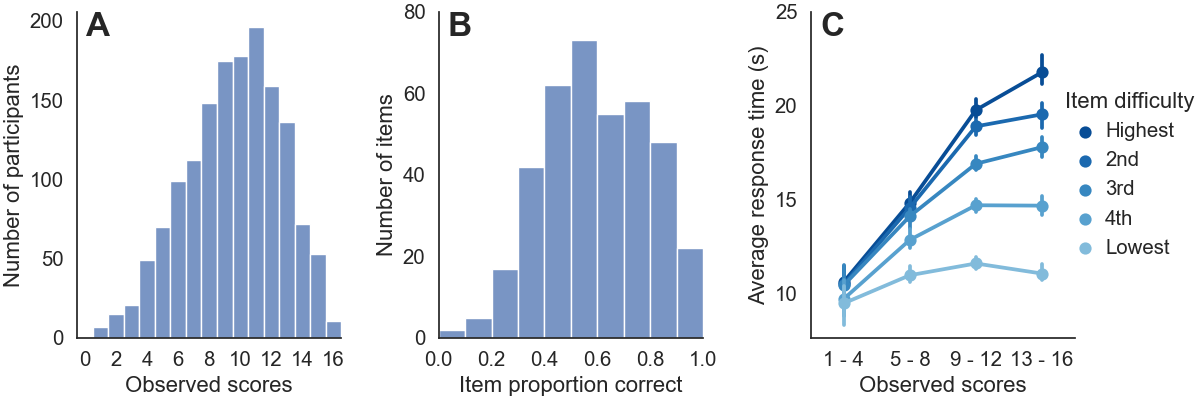
\includegraphics[width=1.0\textwidth]{figures/fig01.png}
\caption{\label{fig:fig01}This is a figure caption.}
\end{figure}
 
Summary paragraph?
 
\subsection{Item response models}

To measure the psychometric properties of each item, we used item response models. Given the hierarchical nature of the MaRs-IB -- 64 items with six variants each -- we specifically modeled participants' response data using item using a series of item cloning models \citep{geerlings2011modeling, cho2014additive, lathrop2017item}. In item cloning models, the variants of an item (or "clones") are explicitly model as having been generated from the same template item (or "family"). The basis of all of the models used here is the three-parameter logistic (3PL) item response model, where the probability of a correct response ($y_{ijk} = 1$) for person $i$ on item clone $k$ belonging to item family $j$ is:

\begin{equation}
p(y_{ijk} = 1) = \gamma_{jk} + (1-\gamma_{jk}) \cdot \text{logit}^{-1} \left( \alpha_{jk} \cdot \theta_i - \beta_{jk} \right)
\end{equation}

\noindent where $\theta_i$ is the latent ability for person $i$, and $\beta_{jk}$, $\alpha_{jk}$, and $\gamma_{jk}$ are the difficulty, discrimination, and guessing parameters for item clone $k$ of item family $j$. Since guessing parameters are challenging to estimate in the absence of very large amounts of data \citep{han2012fixing}, we fixed the guessing parameter for each item clone to the nominal guessing rate ($\gamma_{jk} = 0.25$).

To account for the nested structure of the MaRs-IB, the item difficulty and discrimination parameters were estimated using an additive multilevel item structure model \citep{cho2014additive}. Specifically, the difficulty of item clone $k$ belonging to item family $j$ was expressed as:  

\begin{equation}
\beta_{jk} = \mu_\beta + \sum_{n=1}^N Q_{jn} \delta_{\beta n} + \epsilon_{\beta j} + \sum_{m=1}^M R_{km} \delta_{\beta m} + \epsilon_{\beta k}
\end{equation}

\noindent Every difficulty parameter is thus modeled as an intercept ($\mu_\beta$), reflecting the average difficulty across all items, and four components:

\begin{enumerate}

\item $\sum_{n=1}^N Q_{jn} \delta_{\beta n}$: the effect of the level-1 attributes, where $Q_{jn}$ is the value of attribute $n$ for item family $j$, and $\delta_{\beta n}$ is the effect of attribute $n$. This component is the fixed effects contribution of item family to item difficulty.

\item $\epsilon_{\beta j}$: the level-1 residual, or variance unexplained by the item family attributes. This component is the random effects contribution of item family to item difficulty.

\item $\sum_{m=1}^M R_{km} \delta_{\beta m}$: the effect of the level-2 attributes, where $R_{km}$ is the value of attribute $m$ for item clone $k$, and $\delta_{\beta m}$ is the effect of attribute $m$. This component is the fixed effects contribution of item clone to item difficulty.

\item $\epsilon_{\beta k}$: the level-2 residual, or variance unexplained by the item clone attributes. This component is the random effects contribution of item clone to item difficulty.

\end{enumerate}

To elaborate, level-1 attributes describe the properties of an item family. Here we model the effects of two properties: feature number, or the number of unique shapes in each cell of an item; and rule number, or the number of changing relationships among the shapes (e.g. color change, shape change, position change) a participant must consider in order to solve the item. 

In turn, level-2 attributes describe properties of an item clone. Here we model the effects of two additional properties: distractor type, or whether the distractors were generated following the minimal difference (MD) strategy and a paired difference (PD) strategy; and mean response time, or the average time spent on that item. Mean response time was orthogonalized with respect to the three other item attributes, and therefore reflects any residual structure after accounting for all other modeled effects. 

Similarly, item discrimination parameters were also expressed as the sum of an equivalent set of components:

\begin{equation}
\alpha_{jk} = \mu_\alpha + \sum_{n=1}^N Q_{jn} \delta_{\alpha n} + \epsilon_{\alpha j} + \sum_{m=1}^M R_{km} \delta_{\alpha m} + \epsilon_{\alpha k}
\end{equation}

\noindent The fixed effect components of the item discrimination parameters included the same level-1 and level-2 attributes as for the item difficulty parameters (i.e. number of features, number of rules, distractor type, average response time). During estimation, the item discrimination parameters were restricted to be in the range $\alpha_{jk} \in [0, 5]$.

Though complex, item cloning models provide a natural means of evaluating the success of the MaRs-IB item generation process. For example, modeling an item's properties as a function of its attributes allows us to quantify the extent to which item design worked as intended (e.g. that an increase in the number of changing relationships between shapes corresponds to an increase in item difficulty). The inclusion of level-1 random effects allows us to quantify the extent to which item families with identical attributes (e.g. number of features, number of changing relations) are psychometrically equivalent. Similarly, the inclusion of level-2 random effects allows us to quantify the extent to which clones of an item family are psychometrically equivalent. 

In order to test the hypotheses outlined above, we fit a series of nested item cloning models \citep{cho2014additive, lathrop2017item}: 

\begin{enumerate}

\item \textit{Model a}: Item parameters are expressed only as a function of their level-1 attributes. This model treats all clones within a family as interchangeable and all item families with the same attributes as equivalent. 

\item \textit{Model b}: Item parameters are expressed as a function of their level-1 attributes and residuals. This model treats all clones within a family as interchangeable, but now item families with the same attributes may vary in their properties. 

\item \textit{Model c}: Item parameters are expressed as a function of their level-1 attributes, level-2 attributes, and level-1 residuals. This model allows clones within a family to vary, but all variation must be explained solely through their attributes.  

\item \textit{Model d}: Item parameters are expressed as a function of their level-1/2 attributes residuals. The full model in which item families and clones may vary in their psychometric properties. 

\end{enumerate}

The resulting model fits are then compared as a test of the hypotheses above. For example, if the psychometric properties of items can be solely explained by their attributes, then Model A should be preferred to B; in contrast, if item families psychometrically vary beyond what their attributes can explain, then Model B should be preferred. Similarly, if the clones of an item family are truly equivalent, then Models A or B should be preferred; in contrast, if item clones vary (as a function of their attributes or otherwise) then model C or D should be preferred. 

Finally, we estimated person-level abilities following an explanatory item response modeling approach \citep{wilson2008explanatory}:   

\begin{equation}
\theta_i = \sum_{p=1}^P X_{ip} \rho_p + \epsilon_i    
\end{equation}

\noindent where $X_{ip}$ is the value of attribute $p$ for person $i$, $\rho_p$ is the partial correlation of attribute $n$, and $\epsilon_i$ is variance in ability unexplained by the person-level attributes.

We modeled person-level abilities as a function of four attributes: age, gender (coded as: male = -0.5, female = 0.5; all else = 0), average response time, and $\Delta$ response time. The last term reflected the degree to which a participant adjusted their response time as a function of item difficulty, and thus measured a participant's tendency to slow down (or speed up) in response to more challenging items (Figure \ref{fig:fig01}c).

To ensure the identifiability of all models, person abilities were constrained to have a mean of zero and a variance of 1.0, such that the residual variance was defined as $V(\epsilon) = 1 - \sum \rho_p^2$. Note that all person-level attributes were standard-scored prior being entered into the model.

All models were estimated within a Bayesian framework using Hamiltonian Monte Carlo as implemented in Stan (v2.26) \citep{carpenter2017stan}. For all models, four separate chains with randomised start values each took 7500 samples from the posterior. The first 5000 samples from each chain were discarded. As such, 10,000 post-warmup samples from the joint posterior were retained. The $\hat{R}$ values for all parameters was equal to or less than 1.01, indicating acceptable convergence between chains, and there were no divergent transitions in any chain. 

Models were compared using Bayesian leave-one out cross-validation \citep{vehtari2017practical}, which has been found to perform better than more traditional information criteria for comparing item response models \citep{luo2017performances}. Importantly, we computed the conditional leave-one-cluster out (LOCO) cross- validation \citep{merkle2019bayesian}, which measures a model's ability to generalize to held out items (rather than held out responses). 

The fit of the best-fitting model to the data was evaluated through posterior predictive model checks \citep{gelman1996posterior, levy2017bayesian}. Item fit was assessed using the Orlando and Thissen index ($S-\chi^2$) \citep{toribio2011discrepancy}, which compares the observed and expected proportions of participants who answer an item correctly at each raw-score group. The unidimensionality of the data was assessed using the generalized dimensionality discrepancy measure (GDDM) \citep{levy2011generalized}, which tests for violation of the assumption of local independence. This latter measure is crucial for ensuring there is not non-negligible levels of local item dependence in the data, which may otherwise lower the efficiency of future test forms due to the inclusion of correlated, redundant items.    

\subsection{Model comparison}

First we estimated Models 1-4 holding constant the item discrimination parameters ($\alpha = 1$), which allowed us to investigate the difficulty of MaRs-IB items independently. (Note that these models still included guessing parameters fixed to the nominal guessing rate. We also estimated models with no guessing parameter, i.e. 1PL or Rasch models, but model comparison revealed these to be inferior.) 

The goodness of fit of the four models was compared based on leave-one-cluster out (LOCO) cross-validation as summarized in Table \ref{table:1}. The winning model was Model 1d, in which item difficulties were modeled as a function of all level-1 and level-2 fixed and random effects. This has multiple interpretations, which we will unpack in turn. First, this implies that there was systematic variability in item difficulty at the family-level beyond what could explained by their attributes (this is reflected...

[above to be combined with below when time comes]

First, Model 2 was preferred to Model 1 suggesting that there is variability in the difficulty of item families above and beyond what can be explained by their attributes. Similarly, Model 3 was preferred to Model 2 suggesting that there is systematic variability in the clones of each item family. Finally, Model 4 was preferred to Model 3 suggesting that there is variability in the difficulty of item clones above and beyond what can be explained by their respective attributes. In summary, the full model -- including all fixed and random effect terms -- was preferred to the three simpler models, indicating that item families and clones are nonequivalent even after controlling for their attributes.

The average item difficulty was $\beta_\mu = 0.177$ (95\% HDI = 0.118 - 0.238) but this ranged considerably across items (sd = 1.431, 95\% HDI = 1.370 - 1.492). 


Over half of the variability in item difficulty (65.6\%) was explained by the fixed effects of item family (level-1) and clone (level-2) attributes. The associations between level-1 attributes and item difficulty were as expected: feature number was positively associated with difficulty (beta), such that the inclusion of one additional feature was associated with a 13.1\% reduction in expected accuracy. Similarly, rule number was positively associated with item difficulty (beta), such that the inclusion of one additional rule a 10.1\% reduction in expected accuracy. Turning next to level-2 attributes, distractor type was unexpectedly associated with item difficulty (beta), such that clones with MD distractors clones were associated with a 13.6\% reduction in accuracy compared to clones with PD distractors. This pattern is clearly evident in the raw item-level scores (Figure XX). Finally, average response time was positively associated with difficulty, such that a one standard deviation change in response time was associated with an 11.8\% reduction in accuracy. 

The inclusion of item family (level-1) random effects explained an additional 18.5\% of the variance in item difficulty. In total, the percentage of variance in item difficulty not explained by residual variance from item clones (level-2) was 84.1\%. The residual variance was harder to explain (Figure XXb); indeed, there was no clear patterns in difficulty by item set, suggesting that at least part of residual variance may be explained by idiosynchratic perceptual features of item clones. 

Next we estimated three models as above, but with two key differences: First, we no longer held constant the item discrimination parameters but rather estimated them alongside the item difficulty parameters. Second, whereas the item difficulty parameters were always estimated using the full additive multilevel item structure model (i.e. level-1/2 fixed and random effects), the item discrimination parameters were estimated adding one additional component per model (Model 1: level-1/2 fixed effects only; Model 2: fixed effects and level-1 random effects; Model 3: full model). The goodness of fit of the three models was again compared based on leave-one-cluster out (LOCO) cross-validation as summarized in Table \ref{table:2}. 

First, all three models including discrimination parameters were preferred to the best-fitting model with discrimination parameters held constant. Model 2 was preferred to Model 1 suggesting that there is variability in the discrimination of item families not accounted for by their attributes. Importantly, Model 2 was preferred to Model 3 such that there was insufficient variability in discrimination in item clones to necessitate additional parameters. We return to this point in the Discussion.

Returning to variance partitioning, just less than half of the variance in item discrimination (44.9\%) was explained by attributes of the explained by attributes of item families and clones. Interestingly, only the number of item rules was positively associated with item discrimination (HDI); no other attributes were credibly related (HDIs here). 

Finally, we turn to explanatory item response modeling. The largest effects were from the response times. Average response time blah. Delta response time blah. Interestingly, we found a negative correlation between age and ability, such that older participants tended to perform worse on average. Finally, we observed a small but credible association between gender and ability. Though we used the colorblind stimulus set, it is possible there was residual perceptual difficulty for men compared to women. Granted, this effect is small.

This paragraph should be on fit. Should mention: simulation study, posterior predictive check, item fit indices, and unidimensionality measure. You should probably review a couple of other RPM validation papers to make sure our methods are straight (e.g. doi.org/10.1037/a0027830)

\subsection{Discussion}

In discussing the success of the MaRs-IB generation process, some things to point out:

1. A lot of variance in item difficulty and discrimination can be explained by inherent features of the items. This is great!

2. Though there is quite a bit of residual variance at the item family level, this is fine as we only modeled two features. A point we return to in the Discussion.

3. At the clone level, it seems clear that item clones are not equivalent w.r.t. difficulty. For one thing, MD vs. PD big. Should describe level-2 standard deviation somewhere. 

4. For clone discrimination, it seems less clear. One possibility is that there isn't much variability (cite Embertson). Another possibility is that we are underpowered. Cite Lathrop here for discussion of potential bias.

Summarize as good to go!

\section{Test assembly}

With 64 items, each with six clones, there is a vast universe of possible test forms we could construct. Beginning with our motivating problem -- abbreviated measures of nonverbal reasoning with the potential for retest -- we opted to construct three parallel short form measures. To do so, we used mixed integer programming \citep{der2005wj} to maximize the test information function (TIF) of each short form subject to the following constraints:

\begin{enumerate}

    \item Each short form was required to contain 12 items. This was chosen to minimize administration time of a form (2-4 minutes on average) and to achieve sufficient  reliability (Cronbach's $\alpha \geq 0.8$ in piloting).
    
    \item All short forms were required to be comprised of clones from the same item families. This was chosen to maximize the similarity of the short forms.
    
    \item Assigned clones could be of the MD or PD distractor type, but not both. This was chosen to prevent item overlap, as sometimes the MD and PD distractor strategies generate identical distractors.
    
    \item The difference in TIFs across short forms was required to be minimized. This was chosen to ensure that each short form had similar psychometric properties. 
    
\end{enumerate}

\noindent The TIF was maximized at five ability levels ($\theta = -1.0, -0.5, 0.0, 0.5, 1.0$). Previous simulation studies have shown that target values at three to five well-chosen $\theta$s generally suffice \citep{der2005wj}. Solutions to the mixed integer programming problem were found using the \textit{mip} python package (v1.13.0) \citep{santos2020mixed}.

The test information functions (TIFs) and test characteristic curves (TCCs) for the three short forms are shown in Figure XX. As can be readily observed, the TIFs for each short form are remarkably similar reflecting the constraints of the MIP problem. Thus, the short forms should have similar levels of precision across ability levels. Similarly, the TCCs for each short form are similar, which was by no means guaranteed \citep{ali2016evaluation}. Thus, the short forms are expected to have similar total score distributions.

Thus we proceeded to test each short form. blah blah blah.

\section{Validation Study}

\subsection{Data Collection}

A total of N=347 participants were recruited from the Prolific Academic platform (https://www.prolific.co) to participate in an online behavioral experiment in November, 2021. Participants were eligible if they currently resided in the United States and had not participated in the calibration study. This study was approved by the Institutional Review Board of Princeton University (\#7392), and all participants provided informed consent. Total study duration was approximately 10.8 minutes (4.6 sd) per participant. Participants received monetary compensation for their time (rate USD \$10/hr), plus an incentive-compatible bonus up to \$0.75 based on task performance (average payment: mean = \$2.10 [\$0.18 sd]). 

After providing consent, participants completed the experiment which was divided into three section. In the first, participants completed three short surveys: the 10-item need for cognition survey \citep{chiesi2018applying}, the 8-item PROMIS Cognitive Function-Short Forms (8a) \citep{iverson2021normative}, and the 8-item subject numeracy scale \citep{fagerlin2007measuring}. These measures were included as part of exploratory analyses that were not the central focus of this study and will not be reported in the main text (reported in Supplement). Next, participants completed one of the three 12-item MaRs-IRB short-forms described above. Besides for the items, the administration procedure of the short-forms was identical to that in the Calibration study. Finally, participants completed the 9-item abbreviated Raven's progressive matrices (form A) \citep{bilker2012development}. For consistency's sake, the administration procedure was matched to the MaRs-IB. 

The data from a total of N=47 participants were excluded prior to analysis. Of these, N=17 participants were excluded for having not completed the entire experiment. Separately, the data from N=21 participants were excluded for failing one or more attention checks (infrequency items) embedded in the self-report measures \citep{zorowitz2021inattentive}. The data from N=13 participants were excluded for image loading problems on either the MaRs-IB or RPM tasks. Finally, N=6 participants were excluded for missing or rapid guessing on 4 or more trials during the MaRs-IB or RPM tasks. Note these are not mutually exclusive.

The majority of participants in the validation sample identified as women (men: N=138; women: N=147; non-binary or other: N=13; rather not say: N=2). Participants were 35.0 years old (13.2 sd) on average. The sample was relatively well-educated with the majority having a Bachelor's degree (N=121) or Master's degree or higher (N=45); fewer participants endorsed only completing some college (N=100) or only a high school degree or lower (N=33). 

\subsection{Results}

The distribution of scores on the three MaRs-IB short-forms are summarized in Table \ref{table:2}. Across the short-forms, participants responded correctly on 8.0 of 12 items (sd = 2.5, IQR = 6 - 10). The distribution of scores were skewed towards to higher end, as would be expected given their respective test characteristic curves. A 1-way ANOVA did not reject the null hypothesis that the observed scores across test forms were equal (F(2,97) = 0.253, p = 0.777). Corroborating the predictions from the test assembly, the reliability of each short form was satisfactory (Table \ref{table:2}). 

The distribution of scores on the RPM short-form is similarly summarized in Table \ref{table:2}. On average, participants responded correctly on 4.5 of 9 items (sd = 2.0, IQR = 3 - 9). Scores on the RPM were significantly lower on the RPM than the MaRs-IB ($t = 25.598, p < 1e^{-6}$), indicating that the items on the RPM short-form are more difficult on average than those selected for the MaRs-IB short-forms. The reliability of the measure was similarly good as the MaRs-IB (Table \ref{table:2}). 

To measure convergent validity, blah blah blah. Need to write model here. Or should we write above?

\subsection{Discussion}

\section{General Discussion}

Paragraph XX: item discrimination random effects. Power analysis? also variance explained being similar to literature.

-----
Notes on RT effects: this paragraph should come later, as a discussion point on what we're actually measuring with the MaRs-IB (at least online)

Heitz (2014): in general, an increase in speed comes at the expense of accuracy (speed-accuracy trade-off)

Goldhammer (2015): 

> Individual differences in test performance depend on both between-person differences in speed and ability (i.e., the location of individual speed-ability curves) and the adopted speed-ability compromise within persons (i.e., the location within a speed-ability curve). T

Goldhammer et al. (2015): test takers that increase their work pace have a lower effective ability

> On previous reasoning tasks: "These findings indicate that in tasks that require understanding new problem situations and in which the use of complex cognitive processes is mandatory, higher effective ability is usually associated with lower speed." 

Ranger et al. (2021): 

> Such a relation between response time and response accuracy or between work pace and effective ability is of uttermost importance as it implies that the responses depend on more than just the test taker’s capability.

> the capability is apportioned among two quantities, the effective ability, and the work pace, which constitute the actual performance of a test taker in a test; see Pohl and von Davier (2018) for a discussion on how to describe the performance of test takers. 

As work pace increases, effective ability decreases (irrespective of true capability). Work rate may reflect other processes: persistence, or amount of time before participant gives up, mental effort costs, or foraging costs.  

Basically, summarize results. All points are consistent with dual process theory (automatic vs. controlled processing). suggestins higher ability participants more deliberate, lower ability participants less deliberate. frame from perspective of persistence (ranger 2021).

Need to cite: https://doi.org/10.1016/j.intell.2020.101490

-----

Paragraph XX: future directions modeling speed-accuracy trade-offs

Paragraph XX: model more features as future direction. Carpenter taxonomy. Model by rule type. By perceptual features. automatic item generation as future direction. See \cite{lathrop2017item} for inspiration. Note that this definition of item rules deviates from other established taxonomies of matrix reasoning items \citep{carpenter1990one}, a point we return to in the Discussion.

\bibliography{references}

\begin{table}
    \centering
    \begin{tabular}{c|c|c|c|c|c|c|c}
    \hline
    Model & FE-1 & RE-1 & FE-2 & RE-2 & psis-loco & $\Delta$ psis-loco (se) \\
    \hline
    1a & x &   &   &   & -14516.85 & -1223.69 (44.94)\\
    1b & x & x &   &   & -13804.74 & -511.58 (28.77) \\
    1c & x & x & x &   & -13481.12 & -187.96 (17.25) \\
    1d & x & x & x & x & -13293.16 & - \\
    \hline
    2a & x &   & x &   & -13209.38 & -2.13 (2.04) \\
    2b & x & x & x &   & -13207.25 & - \\
    2c & x & x & x & x & -13208.69 & 1.44 (0.85) \\
    \hline
    \end{tabular}
    \caption{\label{tab:1} Goodness of fit of item response models to MaRs-IB data. Pareto-smoothed importance sampling}
    \label{table:1}
\end{table}

\begin{table}
    \centering
    \begin{tabular}{c|c|c|c}
    Measure & Mean (sd) & IQR & Reliability \\
    \hline
    MaRs-IB SFa & 7.9 (2.4) & 7 - 10 & 0.761 \\
    MaRs-IB SFb & 8.2 (2.6) & 7 - 10 & 0.810 \\
    MaRs-IB SFc & 7.9 (2.7) & 6 - 10 & 0.829 \\
    RPM SFa & 4.5 (2.0) & 3 - 9 & 0.791 \\
    \end{tabular}
    \caption{Caption}
    \label{table:2}
\end{table}

\begin{table}
\begin{center}
\begin{tabular}{lrrrrrr}
\hline
&  Coef. & Std.Err. & z & P$> |$z$|$ & [0.025 & 0.975]  \\
\hline
Intercept &  2.648 &    0.009 & 287.757 &       0.000 &  2.630 &  2.666  \\
accuracy &  0.039 &    0.007 &   5.367 &       0.000 &  0.025 &  0.053  \\
difficulty &  0.073 &    0.005 &  13.292 &       0.000 &  0.062 &  0.083  \\
accuracy:difficulty &  0.097 &    0.007 &  14.351 &       0.000 &  0.084 &  0.110  \\
score &  0.167 &    0.009 &  19.204 &       0.000 &  0.150 &  0.184  \\
accuracy:score & -0.064 &    0.007 &  -8.764 &       0.000 & -0.078 & -0.050  \\
difficulty:score &  0.032 &    0.005 &   6.549 &       0.000 &  0.023 &  0.042  \\
accuracy:difficulty:score &  0.012 &    0.006 &   1.955 &       0.051 & -0.000 &  0.025  \\
\hline
\end{tabular}
\end{center}
\end{table}

\end{document}
